% Deterministic vector renderer for paper/figures/fig-scenario.pdf, v2.
%
% v2 changes against fig-scenario-render.tex:
%   - CUT the actuator icon, the "actuator" label and the rotated "technician at
%     the battery pack" label, freeing 23 bp of width for the columns that carry
%     copy.
%   - CUT the "12 + n/2 cycles" callout. It is Sec. V material and the paper
%     already states it twice.
%   - CUT the three dimension annotations inside the kernel. They were floating
%     labels on leader lines that collided with each other and with the divider.
%     Their content survives twice over: the identity triple in the bottom-left
%     callout, state and provenance in the two request-context boxes that feed
%     the sigma and pi gates.
%   - Type up across the board on the space that freed: senders 7 -> 7.2 bp,
%     outcomes and bottom band 7 -> 7.6 bp, kernel title 7.6 -> 8.2 bp.
%   - Canvas 252x156 -> 252x138. Shorter AND larger type, no overlaps.
%   - The sigma outcome no longer reads "maintenance_mode asserted". The state
%     mask is a positive, monotone precondition (docs/canonical-context.md), so
%     an asserted bit cannot deny anything. The deny is a cleared operating bit.
%
% EVERY box below is sized from a measured typeset dimension, not an estimate.
% Measurements at the stated sizes, in pt, width x (height+depth):
%   badge 7.0            54.9 x  5.1     senders 7.2, 58 bp wide:
%   "Compromised node" bold 7.2 natural width 55.6  -> needs >=58 bp or it wraps
%   sender blocks        54.2 x 27.5     callout 7.6   74.3 x 28.2
%   outcome blocks       47.2 x 20.4     sigma box 7.6 99.4 x 23.5
% If you edit any string, re-measure before trusting the rectangle around it.
%
% Compile from the repository root with:
%   pdflatex -interaction=nonstopmode -halt-on-error -file-line-error \
%     -output-directory=paper/figures -jobname=fig-scenario \
%     paper/figures/fig-scenario-render-v2.tex
\documentclass[tikz,border=0pt]{standalone}
\usepackage[T1]{fontenc}
\usepackage[condensed,sfdefault,type1]{roboto}
\usepackage{pifont}
\usetikzlibrary{arrows.meta,calc,decorations.pathreplacing}

\pdfinfo{
  /Title (Authenticated but unauthorized)
  /Subject (5D H-NGAC authorization scenario)
}

\definecolor{permitfill}{HTML}{A6D6A6}
\definecolor{permitstroke}{HTML}{4A7A4A}
\definecolor{denyfill}{HTML}{F2C4C0}
\definecolor{denystroke}{HTML}{A03030}
\definecolor{transportfill}{HTML}{F7F5F3}
\definecolor{softgray}{HTML}{EEEEEE}
\definecolor{midgray}{HTML}{777777}
\definecolor{ink}{HTML}{202020}

\newcommand{\sendfont}{\fontsize{7.2}{7.2}\selectfont}
\newcommand{\bodyfont}{\fontsize{7.6}{7.6}\selectfont}
\newcommand{\headfont}{\fontsize{8.2}{8.4}\selectfont\bfseries}

\begin{document}
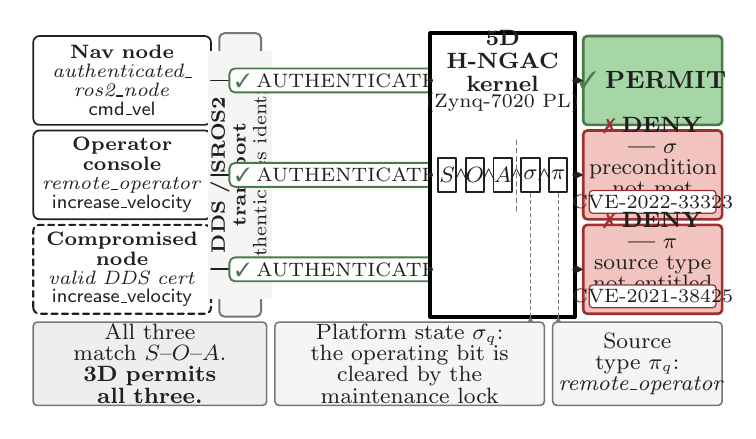
\begin{tikzpicture}[
  x=1bp,
  y=1bp,
  line cap=round,
  line join=round,
  every node/.style={font=\bodyfont,text=ink,inner sep=0.8pt},
  flow/.style={draw=ink,line width=0.62pt,-{Stealth[length=3.2pt,width=3.3pt]}},
  inputflow/.style={draw=midgray,line width=0.55pt,-{Stealth[length=2.8pt,width=2.8pt]}},
  sender/.style={draw=ink,fill=white,line width=0.62pt,rounded corners=2.3pt},
  tag/.style={draw=denystroke,fill=white,line width=0.45pt,rounded corners=1.2pt}
]
  % Exact IEEE single-column width, 252 bp. Height 138 bp = 1.92 in.
  \path[use as bounding box] (0,0) rectangle (252,138);
  \fill[white] (0,0) rectangle (252,138);

  % Three stream heights shared by senders, badges, ports and outcomes:
  % y = 119 (nav), 85 (operator console), 51 (compromised).

  % ---------- Column 1: senders, x 2..66, text width 58 ----------
  \draw[sender] (2,103) rectangle (66,135);
  \node[font=\sendfont,align=center,text width=58pt] at (34,119) {%
    \textbf{Nav node}\\[-0.4pt]
    \textit{authenticated\_}\\[-0.4pt]
    \textit{ros2\_node}\\[-0.4pt]
    \textsf{cmd\_vel}};

  \draw[sender] (2,69) rectangle (66,101);
  \node[font=\sendfont,align=center,text width=58pt] at (34,85) {%
    \textbf{Operator console}\\[-0.4pt]
    \textit{remote\_operator}\\[-0.4pt]
    \textsf{increase\_velocity}};

  \draw[draw=ink,fill=white,line width=0.75pt,dash pattern=on 2.2pt off 1.6pt,
        rounded corners=2.3pt]
    (2,35) rectangle (66,67);
  \node[font=\sendfont,align=center,text width=58pt] at (34,51) {%
    \textbf{Compromised node}\\[-0.4pt]
    \textit{valid DDS cert}\\[-0.4pt]
    \textsf{increase\_velocity}};
  % ---------- Column 2: transport, x 69..84 ----------
  \draw[draw=midgray,fill=transportfill,line width=0.72pt,rounded corners=1.8pt]
    (69,34) rectangle (84,136);
  \node[rotate=90,fill=transportfill,align=center,text width=88pt,
        font=\fontsize{7.4}{7.5}\selectfont]
    at (76.5,85) {\textbf{DDS / SROS2 transport}\\authenticates identity};

  % Three streams. Identical geometry, identical ink, identical badge: the
  % transport layer cannot tell these apart, which is the point of the figure.
  \foreach \yy in {119,85,51}{ \draw[flow] (66,\yy) -- (145,\yy); }
  \foreach \yy in {119,85,51}{
    \node[draw=permitstroke,fill=white,line width=0.68pt,rounded corners=2pt,
          inner xsep=2.2pt,inner ysep=1.8pt,align=center,
          font=\fontsize{7.0}{7.0}\selectfont]
      at (114,\yy) {\textcolor{permitstroke}{\ding{51}}\;AUTHENTICATED};
  }

  % ---------- Column 3: the 5D decision primitive, x 145..197 ----------
  \draw[draw=black,fill=white,line width=1.45pt] (145,34) rectangle (197,136);
  \node[font=\headfont,align=center,text width=48pt] at (171,126)
    {5D H-NGAC\\kernel};
  \node[font=\fontsize{7.0}{7.0}\selectfont] at (171,111) {(Zynq-7020 PL)};

  % Ports make the correspondence with the three outcomes explicit.
  \foreach \yy in {119,85,51}{
    \fill[ink] (145,\yy) circle (0.9pt);
    \fill[ink] (197,\yy) circle (0.9pt);
  }

  % Five gates on the middle stream line. sigma and pi are 32-bit terms sitting
  % beside 256-bit identity terms: extra width in one pipeline stage, not an
  % extra stage. The dashed divider separates the identity triple from the two
  % added dimensions.
  \foreach \xx/\lab in {151/$S$,161/$O$,171/$A$,181/$\sigma$,191/$\pi$}{
    \draw[draw=ink,fill=white,line width=0.7pt] (\xx-3.3,79) rectangle (\xx+3.3,91);
    \node[font=\fontsize{8.0}{8.0}\selectfont\bfseries] at (\xx,85) {\lab};
  }
  \foreach \xx in {156,166,176,186}{
    \node[font=\fontsize{7.0}{7.0}\selectfont] at (\xx,85) {$\wedge$};
  }
  \draw[draw=midgray,line width=0.5pt,dash pattern=on 1.6pt off 1.4pt]
    (176,72) -- (176,98);

  % Request context enters the bottom edge under the gates it feeds.
  \draw[draw=midgray,line width=0.4pt,dash pattern=on 1.2pt off 1.2pt]
    (181,34) -- (181,79);
  \draw[draw=midgray,line width=0.4pt,dash pattern=on 1.2pt off 1.2pt]
    (191,34) -- (191,79);
  \draw[inputflow] (181,32) -- (181,34);
  \draw[inputflow] (191,32) -- (191,34);

  % ---------- Column 4: outcomes, x 200..250, text width 46 ----------
  \draw[draw=permitstroke,fill=permitfill,line width=0.95pt,rounded corners=1.5pt]
    (200,103) rectangle (250,135);
  \node[font=\fontsize{8.6}{8.6}\selectfont\bfseries] at (225,119)
    {\textcolor{permitstroke}{\ding{51}}\;PERMIT};

  \draw[draw=denystroke,fill=denyfill,line width=0.95pt,rounded corners=1.5pt]
    (200,69) rectangle (250,101);
  \node[align=center,text width=46pt] at (225,91.5)
    {\textcolor{denystroke}{\ding{55}}\;\textbf{DENY --- $\sigma$}\\
     precondition not met};
  \draw[tag] (202.2,71.2) rectangle (247.8,79.4);
  \node[font=\fontsize{7.0}{7.0}\selectfont] at (225,75.3) {CVE-2022-33323};

  \draw[draw=denystroke,fill=denyfill,line width=0.95pt,rounded corners=1.5pt]
    (200,35) rectangle (250,67);
  \node[align=center,text width=46pt] at (225,57.5)
    {\textcolor{denystroke}{\ding{55}}\;\textbf{DENY --- $\pi$}\\
     source type not entitled};
  \draw[tag] (202.2,37.2) rectangle (247.8,45.4);
  \node[font=\fontsize{7.0}{7.0}\selectfont] at (225,41.3) {CVE-2021-38425};

  \foreach \yy in {119,85,51}{ \draw[flow] (197,\yy) -- (200,\yy); }

  % ---------- Bottom band, y 2..32 ----------
  % Left: the contrast the paper's claim rests on.
  \draw[draw=midgray,fill=softgray,line width=0.58pt,rounded corners=1.4pt]
    (2,2) rectangle (86,32);
  \node[align=center,text width=80pt] at (44,17)
    {All three match $S$--$O$--$A$.\\\textbf{3D permits all three.}};

  % Right: request context. sigma is a precondition, so the deny above is a
  % cleared operating bit, never an asserted maintenance bit.
  \draw[draw=midgray,fill=transportfill,line width=0.58pt,rounded corners=1.5pt]
    (89,2) rectangle (186,32);
  \node[align=center,text width=93pt] at (137.5,17)
    {Platform state $\sigma_q$: the operating bit is\\cleared by the maintenance lock};
  \draw[draw=midgray,fill=transportfill,line width=0.58pt,rounded corners=1.5pt]
    (189,2) rectangle (250,32);
  \node[align=center,text width=57pt] at (219.5,17)
    {Source type $\pi_q$:\\\textit{remote\_operator}};
\end{tikzpicture}
\end{document}
